\documentclass[twoside]{book}

% Packages required by doxygen
\usepackage{fixltx2e}
\usepackage{calc}
\usepackage{doxygen}
\usepackage[export]{adjustbox} % also loads graphicx
\usepackage{graphicx}
\usepackage[utf8]{inputenc}
\usepackage{makeidx}
\usepackage{multicol}
\usepackage{multirow}
\PassOptionsToPackage{warn}{textcomp}
\usepackage{textcomp}
\usepackage[nointegrals]{wasysym}
\usepackage[table]{xcolor}

% Font selection
\usepackage[T1]{fontenc}
\usepackage[scaled=.90]{helvet}
\usepackage{courier}
\usepackage{amssymb}
\usepackage{sectsty}
\renewcommand{\familydefault}{\sfdefault}
\allsectionsfont{%
  \fontseries{bc}\selectfont%
  \color{darkgray}%
}
\renewcommand{\DoxyLabelFont}{%
  \fontseries{bc}\selectfont%
  \color{darkgray}%
}
\newcommand{\+}{\discretionary{\mbox{\scriptsize$\hookleftarrow$}}{}{}}

% Page & text layout
\usepackage{geometry}
\geometry{%
  a4paper,%
  top=2.5cm,%
  bottom=2.5cm,%
  left=2.5cm,%
  right=2.5cm%
}
\tolerance=750
\hfuzz=15pt
\hbadness=750
\setlength{\emergencystretch}{15pt}
\setlength{\parindent}{0cm}
\setlength{\parskip}{3ex plus 2ex minus 2ex}
\makeatletter
\renewcommand{\paragraph}{%
  \@startsection{paragraph}{4}{0ex}{-1.0ex}{1.0ex}{%
    \normalfont\normalsize\bfseries\SS@parafont%
  }%
}
\renewcommand{\subparagraph}{%
  \@startsection{subparagraph}{5}{0ex}{-1.0ex}{1.0ex}{%
    \normalfont\normalsize\bfseries\SS@subparafont%
  }%
}
\makeatother

% Headers & footers
\usepackage{fancyhdr}
\pagestyle{fancyplain}
\fancyhead[LE]{\fancyplain{}{\bfseries\thepage}}
\fancyhead[CE]{\fancyplain{}{}}
\fancyhead[RE]{\fancyplain{}{\bfseries\leftmark}}
\fancyhead[LO]{\fancyplain{}{\bfseries\rightmark}}
\fancyhead[CO]{\fancyplain{}{}}
\fancyhead[RO]{\fancyplain{}{\bfseries\thepage}}
\fancyfoot[LE]{\fancyplain{}{}}
\fancyfoot[CE]{\fancyplain{}{}}
\fancyfoot[RE]{\fancyplain{}{\bfseries\scriptsize Generated by Doxygen }}
\fancyfoot[LO]{\fancyplain{}{\bfseries\scriptsize Generated by Doxygen }}
\fancyfoot[CO]{\fancyplain{}{}}
\fancyfoot[RO]{\fancyplain{}{}}
\renewcommand{\footrulewidth}{0.4pt}
\renewcommand{\chaptermark}[1]{%
  \markboth{#1}{}%
}
\renewcommand{\sectionmark}[1]{%
  \markright{\thesection\ #1}%
}

% Indices & bibliography
\usepackage{natbib}
\usepackage[titles]{tocloft}
\setcounter{tocdepth}{3}
\setcounter{secnumdepth}{5}
\makeindex

% Hyperlinks (required, but should be loaded last)
\usepackage{ifpdf}
\ifpdf
  \usepackage[pdftex,pagebackref=true]{hyperref}
\else
  \usepackage[ps2pdf,pagebackref=true]{hyperref}
\fi
\hypersetup{%
  colorlinks=true,%
  linkcolor=blue,%
  citecolor=blue,%
  unicode%
}

% Custom commands
\newcommand{\clearemptydoublepage}{%
  \newpage{\pagestyle{empty}\cleardoublepage}%
}

\usepackage{caption}
\captionsetup{labelsep=space,justification=centering,font={bf},singlelinecheck=off,skip=4pt,position=top}

%===== C O N T E N T S =====

\begin{document}

% Titlepage & ToC
\hypersetup{pageanchor=false,
             bookmarksnumbered=true,
             pdfencoding=unicode
            }
\pagenumbering{roman}
\begin{titlepage}
\vspace*{7cm}
\begin{center}%
{\Large My Project }\\
\vspace*{1cm}
{\large Generated by Doxygen 1.8.11}\\
\end{center}
\end{titlepage}
\clearemptydoublepage
\tableofcontents
\clearemptydoublepage
\pagenumbering{arabic}
\hypersetup{pageanchor=true}

%--- Begin generated contents ---
\chapter{Class Index}
\section{Class List}
Here are the classes, structs, unions and interfaces with brief descriptions\+:\begin{DoxyCompactList}
\item\contentsline{section}{\hyperlink{structnode}{node} }{\pageref{structnode}}{}
\item\contentsline{section}{\hyperlink{structnode1}{node1} }{\pageref{structnode1}}{}
\item\contentsline{section}{\hyperlink{structnode__info}{node\+\_\+info} }{\pageref{structnode__info}}{}
\end{DoxyCompactList}

\chapter{File Index}
\section{File List}
Here is a list of all files with brief descriptions\+:\begin{DoxyCompactList}
\item\contentsline{section}{\hyperlink{Lab1_8c}{Lab1.\+c} }{\pageref{Lab1_8c}}{}
\end{DoxyCompactList}

\chapter{Class Documentation}
\hypertarget{structnoArv}{}\section{no\+Arv Struct Reference}
\label{structnoArv}\index{no\+Arv@{no\+Arv}}


Collaboration diagram for no\+Arv\+:
\nopagebreak
\begin{figure}[H]
\begin{center}
\leavevmode
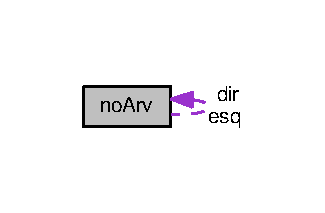
\includegraphics[width=156pt]{structnoArv__coll__graph}
\end{center}
\end{figure}
\subsection*{Public Attributes}
\begin{DoxyCompactItemize}
\item 
int \hyperlink{structnoArv_a024fbe9c9e750cab832562b09d49200e}{info}
\item 
struct \hyperlink{structnoArv}{no\+Arv} $\ast$ \hyperlink{structnoArv_a0c0b5ff0d841e3d90215a04185f0899d}{esq}
\item 
struct \hyperlink{structnoArv}{no\+Arv} $\ast$ \hyperlink{structnoArv_abe103e6775ec6bb1d39b61f54c4cf32c}{dir}
\end{DoxyCompactItemize}


\subsection{Member Data Documentation}
\index{no\+Arv@{no\+Arv}!dir@{dir}}
\index{dir@{dir}!no\+Arv@{no\+Arv}}
\subsubsection[{\texorpdfstring{dir}{dir}}]{\setlength{\rightskip}{0pt plus 5cm}struct {\bf no\+Arv}$\ast$ no\+Arv\+::dir}\hypertarget{structnoArv_abe103e6775ec6bb1d39b61f54c4cf32c}{}\label{structnoArv_abe103e6775ec6bb1d39b61f54c4cf32c}
\index{no\+Arv@{no\+Arv}!esq@{esq}}
\index{esq@{esq}!no\+Arv@{no\+Arv}}
\subsubsection[{\texorpdfstring{esq}{esq}}]{\setlength{\rightskip}{0pt plus 5cm}struct {\bf no\+Arv}$\ast$ no\+Arv\+::esq}\hypertarget{structnoArv_a0c0b5ff0d841e3d90215a04185f0899d}{}\label{structnoArv_a0c0b5ff0d841e3d90215a04185f0899d}
\index{no\+Arv@{no\+Arv}!info@{info}}
\index{info@{info}!no\+Arv@{no\+Arv}}
\subsubsection[{\texorpdfstring{info}{info}}]{\setlength{\rightskip}{0pt plus 5cm}int no\+Arv\+::info}\hypertarget{structnoArv_a024fbe9c9e750cab832562b09d49200e}{}\label{structnoArv_a024fbe9c9e750cab832562b09d49200e}


The documentation for this struct was generated from the following file\+:\begin{DoxyCompactItemize}
\item 
\hyperlink{BinarySearchTree2_8c}{Binary\+Search\+Tree2.\+c}\end{DoxyCompactItemize}

\chapter{File Documentation}
\hypertarget{BinarySearchTree2_8c}{}\section{Binary\+Search\+Tree2.\+c File Reference}
\label{BinarySearchTree2_8c}\index{Binary\+Search\+Tree2.\+c@{Binary\+Search\+Tree2.\+c}}
{\ttfamily \#include $<$stdio.\+h$>$}\\*
{\ttfamily \#include $<$string.\+h$>$}\\*
{\ttfamily \#include $<$ctype.\+h$>$}\\*
{\ttfamily \#include $<$stdlib.\+h$>$}\\*
{\ttfamily \#include $<$math.\+h$>$}\\*
Include dependency graph for Binary\+Search\+Tree2.\+c\+:
\nopagebreak
\begin{figure}[H]
\begin{center}
\leavevmode
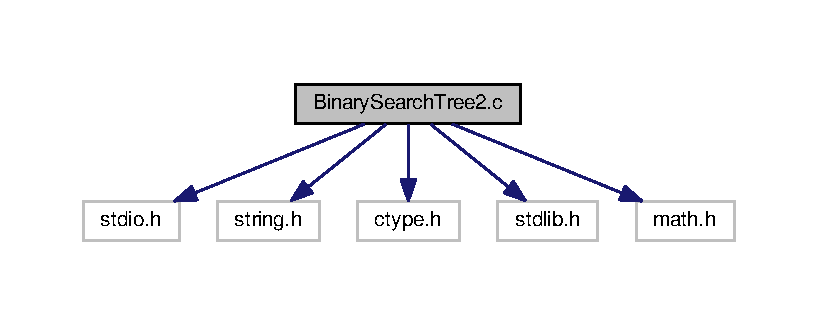
\includegraphics[width=350pt]{BinarySearchTree2_8c__incl}
\end{center}
\end{figure}
\subsection*{Classes}
\begin{DoxyCompactItemize}
\item 
struct \hyperlink{structnoArv}{no\+Arv}
\end{DoxyCompactItemize}
\subsection*{Typedefs}
\begin{DoxyCompactItemize}
\item 
typedef struct \hyperlink{structnoArv}{no\+Arv} \hyperlink{BinarySearchTree2_8c_ab8c46ef838d5fb3bf8ca99827815ecb8}{No\+Arv}
\end{DoxyCompactItemize}
\subsection*{Functions}
\begin{DoxyCompactItemize}
\item 
struct \hyperlink{structnoArv}{no\+Arv} $\ast$ \hyperlink{BinarySearchTree2_8c_a43158fceb90d4d7fe2f1b6d2ab88bca8}{cria} (void)
\item 
struct \hyperlink{structnoArv}{no\+Arv} $\ast$ \hyperlink{BinarySearchTree2_8c_a3fff3326ef764da0c44b10b406a13b91}{retira} (struct \hyperlink{structnoArv}{no\+Arv} $\ast$r, int v)
\item 
void \hyperlink{BinarySearchTree2_8c_a7c7067862fb94194b532586fdfa194b4}{infixa} (\hyperlink{BinarySearchTree2_8c_ab8c46ef838d5fb3bf8ca99827815ecb8}{No\+Arv} $\ast$a)
\item 
void \hyperlink{BinarySearchTree2_8c_ab01995ec05f0ca44ac8d519820428013}{prefixa} (\hyperlink{BinarySearchTree2_8c_ab8c46ef838d5fb3bf8ca99827815ecb8}{No\+Arv} $\ast$a)
\item 
void \hyperlink{BinarySearchTree2_8c_a0c01c8e05f3069616126b9d55438335f}{posfixa} (\hyperlink{BinarySearchTree2_8c_ab8c46ef838d5fb3bf8ca99827815ecb8}{No\+Arv} $\ast$a)
\item 
struct \hyperlink{structnoArv}{no\+Arv} $\ast$ \hyperlink{BinarySearchTree2_8c_a23fc182a29f633a612c4322c44d181fd}{procura} (struct \hyperlink{structnoArv}{no\+Arv} $\ast$r, int v)
\item 
struct \hyperlink{structnoArv}{no\+Arv} $\ast$ \hyperlink{BinarySearchTree2_8c_a6036604c4d3d8262033b6a92fd53b81d}{insere} (struct \hyperlink{structnoArv}{no\+Arv} $\ast$a, int v)
\item 
int \hyperlink{BinarySearchTree2_8c_ae66f6b31b5ad750f1fe042a706a4e3d4}{main} ()
\end{DoxyCompactItemize}
\subsection*{Variables}
\begin{DoxyCompactItemize}
\item 
int \hyperlink{BinarySearchTree2_8c_a13307a0c81bbf19030ea4732534efbec}{aux} = 0
\end{DoxyCompactItemize}


\subsection{Typedef Documentation}
\index{Binary\+Search\+Tree2.\+c@{Binary\+Search\+Tree2.\+c}!No\+Arv@{No\+Arv}}
\index{No\+Arv@{No\+Arv}!Binary\+Search\+Tree2.\+c@{Binary\+Search\+Tree2.\+c}}
\subsubsection[{\texorpdfstring{No\+Arv}{NoArv}}]{\setlength{\rightskip}{0pt plus 5cm}typedef struct {\bf no\+Arv} {\bf No\+Arv}}\hypertarget{BinarySearchTree2_8c_ab8c46ef838d5fb3bf8ca99827815ecb8}{}\label{BinarySearchTree2_8c_ab8c46ef838d5fb3bf8ca99827815ecb8}


\subsection{Function Documentation}
\index{Binary\+Search\+Tree2.\+c@{Binary\+Search\+Tree2.\+c}!cria@{cria}}
\index{cria@{cria}!Binary\+Search\+Tree2.\+c@{Binary\+Search\+Tree2.\+c}}
\subsubsection[{\texorpdfstring{cria(void)}{cria(void)}}]{\setlength{\rightskip}{0pt plus 5cm}struct {\bf no\+Arv}$\ast$ cria (
\begin{DoxyParamCaption}
\item[{void}]{}
\end{DoxyParamCaption}
)}\hypertarget{BinarySearchTree2_8c_a43158fceb90d4d7fe2f1b6d2ab88bca8}{}\label{BinarySearchTree2_8c_a43158fceb90d4d7fe2f1b6d2ab88bca8}

\begin{DoxyCode}
19 \{;
20     \textcolor{keywordflow}{return} NULL;
21 \}
\end{DoxyCode}
\index{Binary\+Search\+Tree2.\+c@{Binary\+Search\+Tree2.\+c}!infixa@{infixa}}
\index{infixa@{infixa}!Binary\+Search\+Tree2.\+c@{Binary\+Search\+Tree2.\+c}}
\subsubsection[{\texorpdfstring{infixa(\+No\+Arv $\ast$a)}{infixa(NoArv *a)}}]{\setlength{\rightskip}{0pt plus 5cm}void infixa (
\begin{DoxyParamCaption}
\item[{{\bf No\+Arv} $\ast$}]{a}
\end{DoxyParamCaption}
)}\hypertarget{BinarySearchTree2_8c_a7c7067862fb94194b532586fdfa194b4}{}\label{BinarySearchTree2_8c_a7c7067862fb94194b532586fdfa194b4}

\begin{DoxyCode}
60 \{
61     \textcolor{keywordflow}{if}(a!=NULL)
62     \{
63         \hyperlink{BinarySearchTree2_8c_a7c7067862fb94194b532586fdfa194b4}{infixa}(a->\hyperlink{structnoArv_a0c0b5ff0d841e3d90215a04185f0899d}{esq});
64         \textcolor{keywordflow}{if}(\hyperlink{BinarySearchTree2_8c_a13307a0c81bbf19030ea4732534efbec}{aux}==1)printf(\textcolor{stringliteral}{" "});
65         printf(\textcolor{stringliteral}{"%d"},a->\hyperlink{structnoArv_a024fbe9c9e750cab832562b09d49200e}{info});
66         \hyperlink{BinarySearchTree2_8c_a13307a0c81bbf19030ea4732534efbec}{aux} = 1;
67         \hyperlink{BinarySearchTree2_8c_a7c7067862fb94194b532586fdfa194b4}{infixa}(a->\hyperlink{structnoArv_abe103e6775ec6bb1d39b61f54c4cf32c}{dir});
68     \}
69 \}
\end{DoxyCode}
\index{Binary\+Search\+Tree2.\+c@{Binary\+Search\+Tree2.\+c}!insere@{insere}}
\index{insere@{insere}!Binary\+Search\+Tree2.\+c@{Binary\+Search\+Tree2.\+c}}
\subsubsection[{\texorpdfstring{insere(struct no\+Arv $\ast$a, int v)}{insere(struct noArv *a, int v)}}]{\setlength{\rightskip}{0pt plus 5cm}struct {\bf no\+Arv}$\ast$ insere (
\begin{DoxyParamCaption}
\item[{struct {\bf no\+Arv} $\ast$}]{a, }
\item[{int}]{v}
\end{DoxyParamCaption}
)}\hypertarget{BinarySearchTree2_8c_a6036604c4d3d8262033b6a92fd53b81d}{}\label{BinarySearchTree2_8c_a6036604c4d3d8262033b6a92fd53b81d}

\begin{DoxyCode}
104 \{
105     \textcolor{keywordflow}{if}(a==NULL)
106     \{
107         a = (\hyperlink{structnoArv}{NoArv}*)malloc(\textcolor{keyword}{sizeof}(\textcolor{keyword}{struct} \hyperlink{structnoArv}{noArv}));
108         a->\hyperlink{structnoArv_a024fbe9c9e750cab832562b09d49200e}{info} = v;
109         a->\hyperlink{structnoArv_a0c0b5ff0d841e3d90215a04185f0899d}{esq} = a->\hyperlink{structnoArv_abe103e6775ec6bb1d39b61f54c4cf32c}{dir} = NULL;
110     \}
111     \textcolor{keywordflow}{else} \textcolor{keywordflow}{if}(v<a->\hyperlink{structnoArv_a024fbe9c9e750cab832562b09d49200e}{info})a->\hyperlink{structnoArv_a0c0b5ff0d841e3d90215a04185f0899d}{esq} = \hyperlink{BinarySearchTree2_8c_a6036604c4d3d8262033b6a92fd53b81d}{insere}(a->\hyperlink{structnoArv_a0c0b5ff0d841e3d90215a04185f0899d}{esq},v);
112     \textcolor{keywordflow}{else} \textcolor{keywordflow}{if}(v>a->\hyperlink{structnoArv_a024fbe9c9e750cab832562b09d49200e}{info})a->\hyperlink{structnoArv_abe103e6775ec6bb1d39b61f54c4cf32c}{dir} = \hyperlink{BinarySearchTree2_8c_a6036604c4d3d8262033b6a92fd53b81d}{insere}(a->\hyperlink{structnoArv_abe103e6775ec6bb1d39b61f54c4cf32c}{dir},v);
113     \textcolor{keywordflow}{return} a;
114 \}
\end{DoxyCode}
\index{Binary\+Search\+Tree2.\+c@{Binary\+Search\+Tree2.\+c}!main@{main}}
\index{main@{main}!Binary\+Search\+Tree2.\+c@{Binary\+Search\+Tree2.\+c}}
\subsubsection[{\texorpdfstring{main()}{main()}}]{\setlength{\rightskip}{0pt plus 5cm}int main (
\begin{DoxyParamCaption}
{}
\end{DoxyParamCaption}
)}\hypertarget{BinarySearchTree2_8c_ae66f6b31b5ad750f1fe042a706a4e3d4}{}\label{BinarySearchTree2_8c_ae66f6b31b5ad750f1fe042a706a4e3d4}

\begin{DoxyCode}
117 \{
118     \textcolor{keyword}{struct }\hyperlink{structnoArv}{noArv} *g = \hyperlink{BinarySearchTree2_8c_a43158fceb90d4d7fe2f1b6d2ab88bca8}{cria}();
119     \textcolor{keywordtype}{char} str[10];
120     \textcolor{keywordtype}{int} x;
121     \textcolor{keywordflow}{while}(scanf(\textcolor{stringliteral}{"%[^\(\backslash\)n]s"},str)!=EOF)
122     \{
123         \textcolor{keywordflow}{if}(str[0]==\textcolor{charliteral}{'I'} && str[1]==\textcolor{charliteral}{' '})\{
124             x = atoi(&str[2]);
125             g = \hyperlink{BinarySearchTree2_8c_a6036604c4d3d8262033b6a92fd53b81d}{insere}(g,x);
126         \}
127         \textcolor{keywordflow}{if}(str[0]==\textcolor{charliteral}{'P'} && str[1]==\textcolor{charliteral}{' '})\{
128             x = atoi(&str[2]);
129             \textcolor{keywordflow}{if}(\hyperlink{BinarySearchTree2_8c_a23fc182a29f633a612c4322c44d181fd}{procura}(g,x))printf(\textcolor{stringliteral}{"%d existe\(\backslash\)n"},x);
130             \textcolor{keywordflow}{else} printf(\textcolor{stringliteral}{"%d nao existe\(\backslash\)n"},x);
131         \}
132         \textcolor{keywordflow}{if}(str[0]==\textcolor{charliteral}{'I'} && str[1]==\textcolor{charliteral}{'N'})\{
133             \hyperlink{BinarySearchTree2_8c_a13307a0c81bbf19030ea4732534efbec}{aux} = 0;
134             \hyperlink{BinarySearchTree2_8c_a7c7067862fb94194b532586fdfa194b4}{infixa}(g);
135             printf(\textcolor{stringliteral}{"\(\backslash\)n"});
136         \}
137         \textcolor{keywordflow}{if}(str[0]==\textcolor{charliteral}{'P'} && str[1]==\textcolor{charliteral}{'O'})\{
138             \hyperlink{BinarySearchTree2_8c_a13307a0c81bbf19030ea4732534efbec}{aux} = 0;
139             \hyperlink{BinarySearchTree2_8c_a0c01c8e05f3069616126b9d55438335f}{posfixa}(g);
140             printf(\textcolor{stringliteral}{"\(\backslash\)n"});
141         \}
142         \textcolor{keywordflow}{if}(str[0]==\textcolor{charliteral}{'P'} && str[1]==\textcolor{charliteral}{'R'})\{
143             \hyperlink{BinarySearchTree2_8c_a13307a0c81bbf19030ea4732534efbec}{aux} = 0;
144             \hyperlink{BinarySearchTree2_8c_ab01995ec05f0ca44ac8d519820428013}{prefixa}(g);
145             printf(\textcolor{stringliteral}{"\(\backslash\)n"});
146         \}
147         \textcolor{keywordflow}{if}(str[0]==\textcolor{charliteral}{'R'})
148         \{
149             x = atoi(&str[2]);
150             g = \hyperlink{BinarySearchTree2_8c_a3fff3326ef764da0c44b10b406a13b91}{retira}(g,x);
151         \}
152         getchar();
153     \}
154     \textcolor{keywordflow}{return} 0;
155 \}\end{DoxyCode}


Here is the call graph for this function\+:
\nopagebreak
\begin{figure}[H]
\begin{center}
\leavevmode
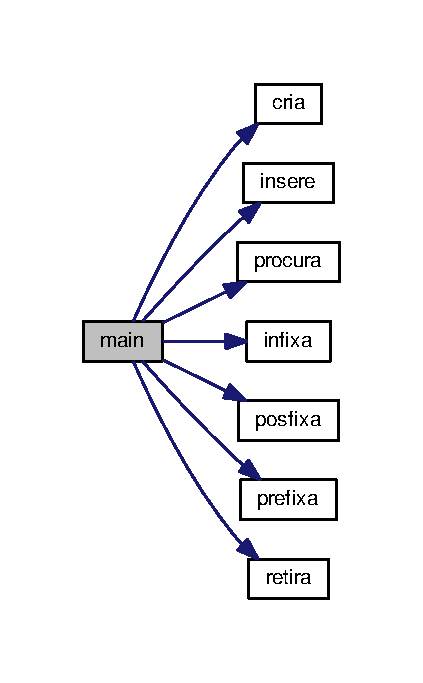
\includegraphics[width=203pt]{BinarySearchTree2_8c_ae66f6b31b5ad750f1fe042a706a4e3d4_cgraph}
\end{center}
\end{figure}


\index{Binary\+Search\+Tree2.\+c@{Binary\+Search\+Tree2.\+c}!posfixa@{posfixa}}
\index{posfixa@{posfixa}!Binary\+Search\+Tree2.\+c@{Binary\+Search\+Tree2.\+c}}
\subsubsection[{\texorpdfstring{posfixa(\+No\+Arv $\ast$a)}{posfixa(NoArv *a)}}]{\setlength{\rightskip}{0pt plus 5cm}void posfixa (
\begin{DoxyParamCaption}
\item[{{\bf No\+Arv} $\ast$}]{a}
\end{DoxyParamCaption}
)}\hypertarget{BinarySearchTree2_8c_a0c01c8e05f3069616126b9d55438335f}{}\label{BinarySearchTree2_8c_a0c01c8e05f3069616126b9d55438335f}

\begin{DoxyCode}
83 \{
84     \textcolor{keywordflow}{if}(a!=NULL)
85     \{
86 
87         \hyperlink{BinarySearchTree2_8c_a0c01c8e05f3069616126b9d55438335f}{posfixa}(a->\hyperlink{structnoArv_a0c0b5ff0d841e3d90215a04185f0899d}{esq});
88         \hyperlink{BinarySearchTree2_8c_a0c01c8e05f3069616126b9d55438335f}{posfixa}(a->\hyperlink{structnoArv_abe103e6775ec6bb1d39b61f54c4cf32c}{dir});
89         \textcolor{keywordflow}{if}(\hyperlink{BinarySearchTree2_8c_a13307a0c81bbf19030ea4732534efbec}{aux}==1)printf(\textcolor{stringliteral}{" "});
90         printf(\textcolor{stringliteral}{"%d"},a->\hyperlink{structnoArv_a024fbe9c9e750cab832562b09d49200e}{info});
91         \hyperlink{BinarySearchTree2_8c_a13307a0c81bbf19030ea4732534efbec}{aux} = 1;
92     \}
93 \}
\end{DoxyCode}
\index{Binary\+Search\+Tree2.\+c@{Binary\+Search\+Tree2.\+c}!prefixa@{prefixa}}
\index{prefixa@{prefixa}!Binary\+Search\+Tree2.\+c@{Binary\+Search\+Tree2.\+c}}
\subsubsection[{\texorpdfstring{prefixa(\+No\+Arv $\ast$a)}{prefixa(NoArv *a)}}]{\setlength{\rightskip}{0pt plus 5cm}void prefixa (
\begin{DoxyParamCaption}
\item[{{\bf No\+Arv} $\ast$}]{a}
\end{DoxyParamCaption}
)}\hypertarget{BinarySearchTree2_8c_ab01995ec05f0ca44ac8d519820428013}{}\label{BinarySearchTree2_8c_ab01995ec05f0ca44ac8d519820428013}

\begin{DoxyCode}
72 \{
73     \textcolor{keywordflow}{if}(a!=NULL)
74     \{
75         \textcolor{keywordflow}{if}(\hyperlink{BinarySearchTree2_8c_a13307a0c81bbf19030ea4732534efbec}{aux}==1)printf(\textcolor{stringliteral}{" "});
76         printf(\textcolor{stringliteral}{"%d"},a->\hyperlink{structnoArv_a024fbe9c9e750cab832562b09d49200e}{info});
77         \hyperlink{BinarySearchTree2_8c_a13307a0c81bbf19030ea4732534efbec}{aux} = 1;
78         \hyperlink{BinarySearchTree2_8c_ab01995ec05f0ca44ac8d519820428013}{prefixa}(a->\hyperlink{structnoArv_a0c0b5ff0d841e3d90215a04185f0899d}{esq});
79         \hyperlink{BinarySearchTree2_8c_ab01995ec05f0ca44ac8d519820428013}{prefixa}(a->\hyperlink{structnoArv_abe103e6775ec6bb1d39b61f54c4cf32c}{dir});
80     \}
81 \}
\end{DoxyCode}
\index{Binary\+Search\+Tree2.\+c@{Binary\+Search\+Tree2.\+c}!procura@{procura}}
\index{procura@{procura}!Binary\+Search\+Tree2.\+c@{Binary\+Search\+Tree2.\+c}}
\subsubsection[{\texorpdfstring{procura(struct no\+Arv $\ast$r, int v)}{procura(struct noArv *r, int v)}}]{\setlength{\rightskip}{0pt plus 5cm}struct {\bf no\+Arv}$\ast$ procura (
\begin{DoxyParamCaption}
\item[{struct {\bf no\+Arv} $\ast$}]{r, }
\item[{int}]{v}
\end{DoxyParamCaption}
)}\hypertarget{BinarySearchTree2_8c_a23fc182a29f633a612c4322c44d181fd}{}\label{BinarySearchTree2_8c_a23fc182a29f633a612c4322c44d181fd}

\begin{DoxyCode}
95 \{
96     \textcolor{keywordflow}{if}(r==NULL)
97         \textcolor{keywordflow}{return} NULL;
98     \textcolor{keywordflow}{else} \textcolor{keywordflow}{if}(r->\hyperlink{structnoArv_a024fbe9c9e750cab832562b09d49200e}{info}>v)\textcolor{keywordflow}{return} \hyperlink{BinarySearchTree2_8c_a23fc182a29f633a612c4322c44d181fd}{procura}(r->\hyperlink{structnoArv_a0c0b5ff0d841e3d90215a04185f0899d}{esq},v);
99     \textcolor{keywordflow}{else} \textcolor{keywordflow}{if}(r->\hyperlink{structnoArv_a024fbe9c9e750cab832562b09d49200e}{info}<v)\textcolor{keywordflow}{return} \hyperlink{BinarySearchTree2_8c_a23fc182a29f633a612c4322c44d181fd}{procura}(r->\hyperlink{structnoArv_abe103e6775ec6bb1d39b61f54c4cf32c}{dir},v);
100     \textcolor{keywordflow}{else} \textcolor{keywordflow}{return} r;
101 \}
\end{DoxyCode}
\index{Binary\+Search\+Tree2.\+c@{Binary\+Search\+Tree2.\+c}!retira@{retira}}
\index{retira@{retira}!Binary\+Search\+Tree2.\+c@{Binary\+Search\+Tree2.\+c}}
\subsubsection[{\texorpdfstring{retira(struct no\+Arv $\ast$r, int v)}{retira(struct noArv *r, int v)}}]{\setlength{\rightskip}{0pt plus 5cm}struct {\bf no\+Arv}$\ast$ retira (
\begin{DoxyParamCaption}
\item[{struct {\bf no\+Arv} $\ast$}]{r, }
\item[{int}]{v}
\end{DoxyParamCaption}
)}\hypertarget{BinarySearchTree2_8c_a3fff3326ef764da0c44b10b406a13b91}{}\label{BinarySearchTree2_8c_a3fff3326ef764da0c44b10b406a13b91}

\begin{DoxyCode}
23 \{
24     \textcolor{keywordflow}{if}(r==NULL)\textcolor{keywordflow}{return} NULL;
25     \textcolor{keywordflow}{else} \textcolor{keywordflow}{if}(r->\hyperlink{structnoArv_a024fbe9c9e750cab832562b09d49200e}{info} > v)r->\hyperlink{structnoArv_a0c0b5ff0d841e3d90215a04185f0899d}{esq} = \hyperlink{BinarySearchTree2_8c_a3fff3326ef764da0c44b10b406a13b91}{retira}(r->\hyperlink{structnoArv_a0c0b5ff0d841e3d90215a04185f0899d}{esq},v);
26     \textcolor{keywordflow}{else} \textcolor{keywordflow}{if}(r->\hyperlink{structnoArv_a024fbe9c9e750cab832562b09d49200e}{info} < v)r->\hyperlink{structnoArv_abe103e6775ec6bb1d39b61f54c4cf32c}{dir} = \hyperlink{BinarySearchTree2_8c_a3fff3326ef764da0c44b10b406a13b91}{retira}(r->\hyperlink{structnoArv_abe103e6775ec6bb1d39b61f54c4cf32c}{dir},v);
27     \textcolor{keywordflow}{else}\{
28         \textcolor{keywordflow}{if}(r->\hyperlink{structnoArv_a0c0b5ff0d841e3d90215a04185f0899d}{esq} == NULL && r->\hyperlink{structnoArv_abe103e6775ec6bb1d39b61f54c4cf32c}{dir} ==NULL)
29         \{
30             free(r);
31             r = NULL;
32         \}
33         \textcolor{keywordflow}{else} \textcolor{keywordflow}{if}(r->\hyperlink{structnoArv_a0c0b5ff0d841e3d90215a04185f0899d}{esq} == NULL)
34         \{
35             \hyperlink{structnoArv}{NoArv} *t = r;
36             r = r->\hyperlink{structnoArv_abe103e6775ec6bb1d39b61f54c4cf32c}{dir};
37             free(t);
38         \}
39         \textcolor{keywordflow}{else} \textcolor{keywordflow}{if}(r->\hyperlink{structnoArv_abe103e6775ec6bb1d39b61f54c4cf32c}{dir}==NULL)
40         \{
41             \hyperlink{structnoArv}{NoArv}* t = r;
42             r = r->\hyperlink{structnoArv_a0c0b5ff0d841e3d90215a04185f0899d}{esq};
43             free(t);
44         \}
45         \textcolor{keywordflow}{else}\{
46             \hyperlink{structnoArv}{NoArv}* f = r->\hyperlink{structnoArv_a0c0b5ff0d841e3d90215a04185f0899d}{esq};
47             \textcolor{keywordflow}{while}(f->\hyperlink{structnoArv_abe103e6775ec6bb1d39b61f54c4cf32c}{dir} !=NULL)
48             \{
49                 f = f->\hyperlink{structnoArv_abe103e6775ec6bb1d39b61f54c4cf32c}{dir};
50             \}
51             r->\hyperlink{structnoArv_a024fbe9c9e750cab832562b09d49200e}{info} = f->\hyperlink{structnoArv_a024fbe9c9e750cab832562b09d49200e}{info};
52             f->\hyperlink{structnoArv_a024fbe9c9e750cab832562b09d49200e}{info} = v;
53             r->\hyperlink{structnoArv_a0c0b5ff0d841e3d90215a04185f0899d}{esq} = \hyperlink{BinarySearchTree2_8c_a3fff3326ef764da0c44b10b406a13b91}{retira}(r->\hyperlink{structnoArv_a0c0b5ff0d841e3d90215a04185f0899d}{esq},v);
54         \}
55 
56     \}
57     \textcolor{keywordflow}{return} r;
58 \}
\end{DoxyCode}


\subsection{Variable Documentation}
\index{Binary\+Search\+Tree2.\+c@{Binary\+Search\+Tree2.\+c}!aux@{aux}}
\index{aux@{aux}!Binary\+Search\+Tree2.\+c@{Binary\+Search\+Tree2.\+c}}
\subsubsection[{\texorpdfstring{aux}{aux}}]{\setlength{\rightskip}{0pt plus 5cm}int aux = 0}\hypertarget{BinarySearchTree2_8c_a13307a0c81bbf19030ea4732534efbec}{}\label{BinarySearchTree2_8c_a13307a0c81bbf19030ea4732534efbec}

%--- End generated contents ---

% Index
\backmatter
\newpage
\phantomsection
\clearemptydoublepage
\addcontentsline{toc}{chapter}{Index}
\printindex

\end{document}
